\chapter*{Introduzione}
Definiamo un grafo come una coppia formata da \textbf{nodi} e \textbf{archi/spigoli}\footnote{Nel caso in cui il grafo è orientato si parlo di archi, altrimenti di spigoli.}. Questo, si indica tipicamente come $G=(V,E)$ con $V$ l'insieme dei nodi e $E$ l'insieme degli archi.
Definiamo un \textbf{grafo semplice} un grafo privo di cappi (archi verso sé stesso) o archi multipli (archi che collegano gli stessi vertici nello stesso verso). 
Sia $e=(x_1,x_2)$, diremo che $x_1$ e $x_2$ sono \textbf{adiacenti}. Nel caso dei grafi orientati questa situazione si complica un po' a causa del fatto che non è detto che se esiste $e_1=(x_1,x_2)$ esiste anche $e_2=(x_2,x_1)$. 
Sia $G=(V,E)$ un grafo orientato, si definisce \textbf{grafo trasposto} $G^T = \{(u,v): u,v \in V, (v,u)\in E\}$, cioè è lo stesso grafo ma con gli archi con verso invertito. 
\begin{figure}[H]
    \centering
    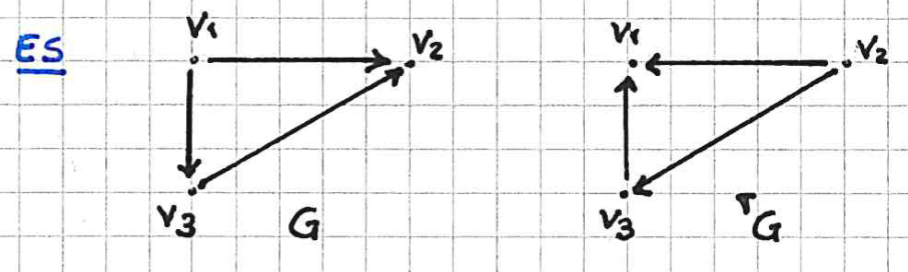
\includegraphics[width=0.6\linewidth]{Images/capitolo_1/trasposto.png}
\end{figure}
Definiamo un \textbf{intorno aperto o open neighborhood} di un vertice l'inseme:
\[N(u)=\{v \in V :(u,v)\in S\}\]
Parliamo, invece, di \textbf{intorno chiuso} l'insieme:
\[N[u] = \{u\} \cup N(u) \]
\begin{figure}[H]
    \centering
    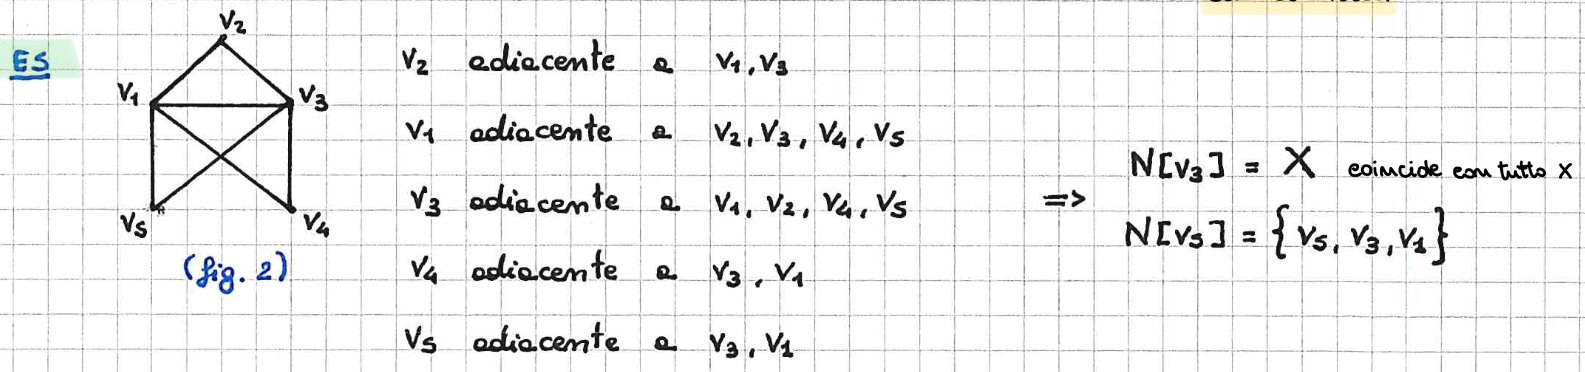
\includegraphics[width=0.6\linewidth]{Images/capitolo_1/neighborhood.png}
\end{figure}

Sia $G=(V,E)$ un grafo, si dice che \textbf{u domina v} se $N[v] \subseteq N[u]$, cioè \textbf{u è adiacente a tutti i vertici adiacenti a v}.
Definiamo un nodo come \textbf{nodo universale} se questo è \textbf{adiacente a tutti i nodi del grafo}.\\
Sia $D \subseteq V$, si dice che $D$ è \textbf{dominante} se $N[D] = \bigcup N[v] = V$  cioè se tutti i nodi appartenenti all'insieme uniti hanno come vertici adiacenti tutti i vertici del grafo. La più piccola cardinalità di un insieme dominante è detta \textbf{numero dominante}. \\
Se in un grafo G, ogni vertice è adiacente a tutti gli altri, diciamo che \textbf{G è completo} e lo indicheremo come $K_n$ dove n è il numero di vertici.\\
Definiamo il \textbf{grado di un vertice} il numero di spigoli incidenti al vertice. Indichiamo questo valore con $d(v)$. 
Indicheremo come \textbf{grado massimo} $\Delta(G)$ il massimo grado di un vertice nel grafo. Allo stesso modo facciamo con il \textbf{grado minimo} indicato con $\delta(G)$.
Nel caso di grafi orientati faremo riferimento al \textbf{grado entrante} $d_e(v)$ come il numero di archi entranti in v e al \textbf{grado uscente} $d_u(v)$ come il numero di archi uscenti da v. 
In futuro vedremo come un nodo con soli archi uscenti è una \textbf{sorgente} mentre un nodo con soli archi entranti è un \textbf{pozzo}.\\
Parleremo di \textbf{grafi orientati pesati} se, a ogni arco o nodo sono associati dei pesi $w$. Nel caso in cui il peso è associato all'arco, allora $w: E \rightarrow R$, altrimenti  $w: V \rightarrow R$.